\documentclass[a4paper,10pt]{article}
\usepackage{fullpage}
\usepackage{float}
\usepackage[english]{babel}
\usepackage{graphicx,subfig,wrapfig}
\usepackage{amsmath,amsfonts,amsthm,amssymb} 
\usepackage{fancyhdr,fancybox,color}
\usepackage{epstopdf}
\usepackage{enumerate}
\usepackage[amssymb]{SIunits}             	% SI units package
\definecolor{MyBlue}{rgb}{0,0.3,0.6}      	
\usepackage[colorlinks=true,linkcolor=MyBlue,plainpages=false,citecolor=MyBlue,urlcolor=MyBlue]{hyperref}
\usepackage[all]{hypcap}   					%fixes the hyperref, such that links are anchored at the bottom of the images, not the top
\usepackage{natbib}

\nonfrenchspacing

\begin{document} 
\thispagestyle{empty} % remove the page number on this page

\noindent Chair: Physics of Fluids group
\begin{center}
 \begin{LARGE}
 Sliding of oil-engulfed droplets
 \end{LARGE}
\end{center}

\section*{Project description}
The sight of rain droplets sticking to window panes is fairly ubiquitous. Upon closer inspection, one can see that sometimes the droplets stick, whereas on other occasions they slide. While sticky droplets may be fine on a window pane, they can be quite a nuisance on the windshield of a car or on the lenses of prescription glasses. One way to get rid of this droplets is to make the surface slippery by coating it with a thin layer of a transparent oil. This facilitates gravity-driven sliding of the water droplet. In such a situation, depending on the interfacial tensions, the oil may completely engulf the water droplet (as shown in Fig.~\ref{figure}). However, how this engulfment affects the sliding behavior of the water droplet is not yet fully understood. In this work, we will experimentally and/or numerically study the sliding behavior of water droplets engulfed by an oil layer. 

\begin{figure}[h]
\centering
\includegraphics[width=0.75\textwidth]{engulfed_droplet.eps}
\caption{Water droplet engulfed by an oil layer (adapted from~\cite{li-2020-pnas}).}
\label{figure}
\end{figure}


\section*{What are the learning components?}
Learning expectations are two-fold; (i) familiarity with the state-of-the-art simulation code, Basilisk C. (ii) Hands-on experience with experimental methods and equipment at the host group.\\

\noindent Specifically, the intern will learn

\begin{enumerate}
	\item volume of fluid (VoF) numerical simulation using Basilisk C to model sliding of droplets
	\item setting up experiments involving state-of-the-art high-speed imaging
	\item modeling and analyzing four-phase systems with multiple three-phase contact lines. 
	\item handling pinning and sliding in these multi-phase systems
\end{enumerate}

\noindent {\it Soft skills:}

\noindent After from the above-mentioned technical skills, the intern will also develop a range of soft skills. The internship will not only expose them to learn crucial research techniques but also give them a foreign exposure. At the end of the internship, they will have a knack to work effectively with other people from various ethnic, educational, and work experience backgrounds. This will help them later in the undergraduate studies as well as get a Ph.D. position at a distinguished group.

\section*{What will the intern do?}
In the Physics of Fluids group, we are looking for enthusiastic students to join our newly established project on sliding of oil-engulfed droplets.
\begin{enumerate}
	\item They will study wetting phenomena in 4-phase systems, precursor films, and viscous dissipation. 
	\item They will work with experimentalists and numericists. 
	\item They will get hands-on experience on experiments involving state-of-the-art high-speed imaging.
	\item They will work with the Computational Fluid Dynamics (CFD) fundamentals, and use the free software program Basilisk C \href{http://basilisk.dalembert.upmc.fr}{(http://basilisk.dalembert.upmc.fr)}.
	\item They will undertake basic and advanced scientific data analysis.
\end{enumerate}

\section*{Future perspectives}

The training period will help develop substantive knowledge in dynamics of droplets and will strengthen the fundamentals of direct numerical simulations. The Physics of Fluids chair at the University of Twente hosts one of the biggest international personnel (including Ph.D. students and postdocs) and has a strong reputation at an international stage. The intern will be introduced to how research is conducted and evaluated in the area of droplet phenomenon. The intern will also learn to demonstrate their ability to communicate the result of his research in an efficient manner. These essential skills will give them an exposure to doctoral research and will be helpful for him to pursue doctoral studies after graduation.


\section*{Project timeline}
\begin{figure}[H]
	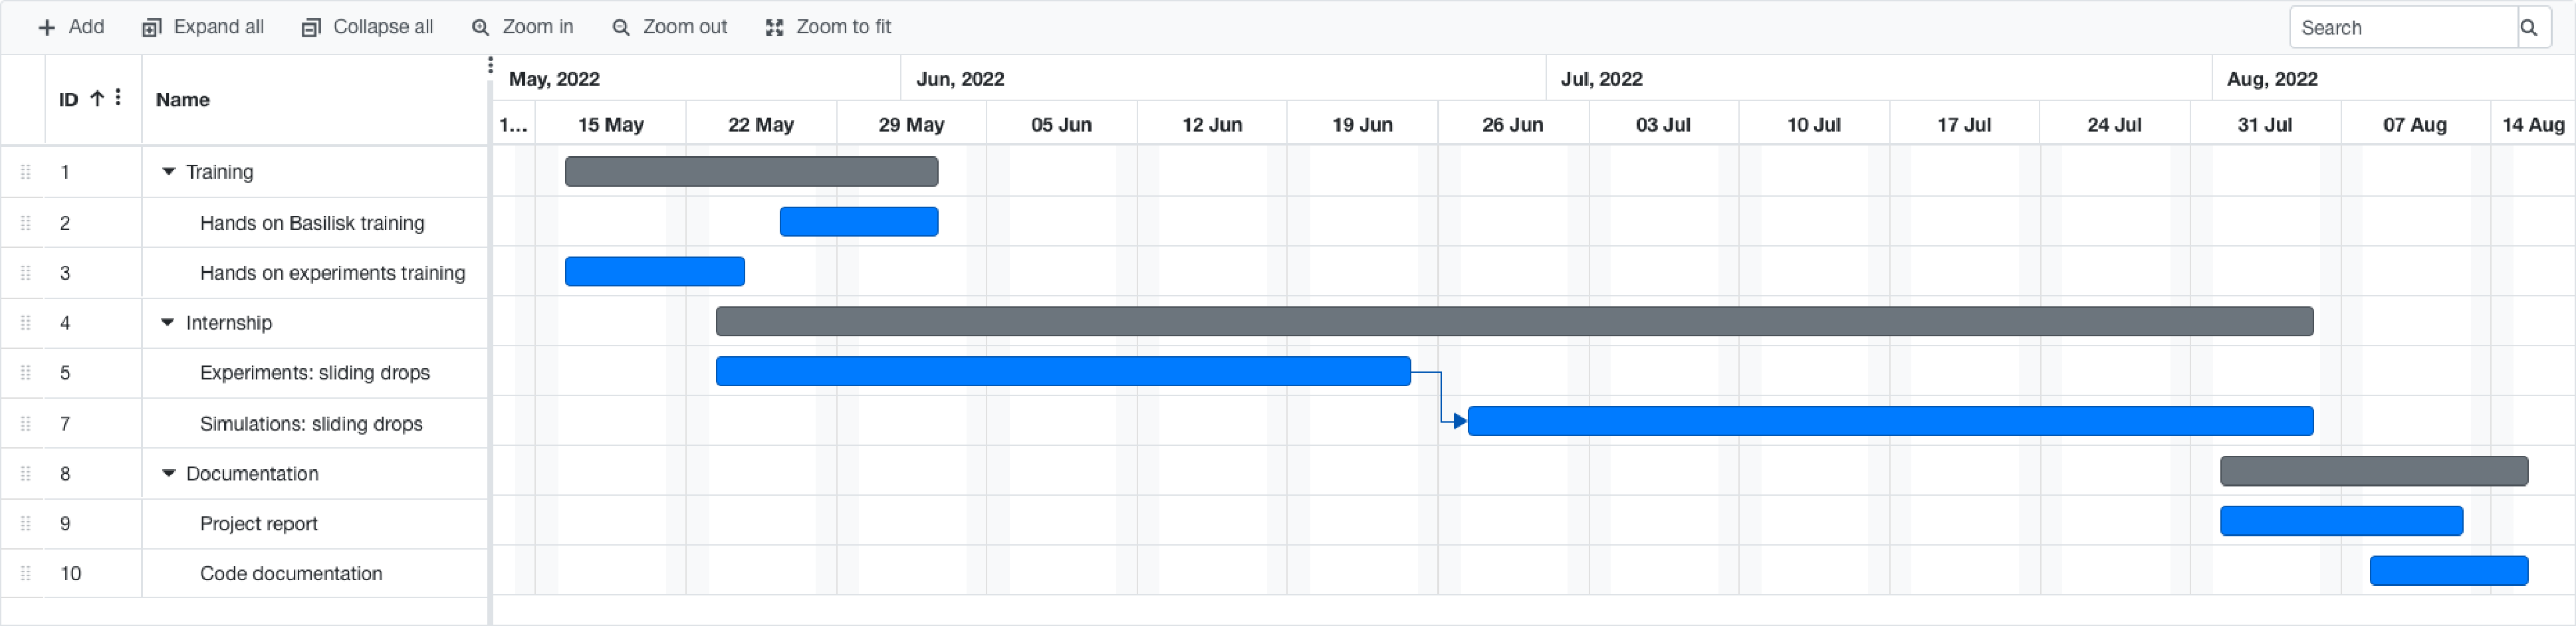
\includegraphics[width=\textwidth]{OnlineGantt2022045.pdf}
	\caption{Timeline and trainee program}
\end{figure}

\section*{Host personnel}

For any questions, please feel free to contact Uddalok Sen (experiments) or Vatsal Sanjay (numerics); details below: 

\begin{center}
	\begin{tabular}{|l|l|l|l|}
		\hline \textbf{Supervision} & \textbf{E-mail} & \textbf{Tel.} & \textbf{Office} \\ 
		\hline Vatsal Sanjay & \href{mailto:contact@vatsalsanjay.com}{contact@vatsalsanjay.com} & +31 687668747/+91 7895940240 & Meander 246B \\ 
		\hline Dr. Uddalok (Udo) Sen & \href{mailto:u.sen@utwente.nl}{u.sen@utwente.nl} & +31 53 489 9064 & Meander 214B \\ 
		\hline Prof. Dr. Detlef Lohse & \href{mailto:d.lohse@utwente.nl}{d.lohse@utwente.nl} & +31 53 489 8076 & Meander 261 \\ 
		\hline 
	\end{tabular} 
\end{center}

\pagebreak

\vspace{20mm}

\noindent Sign: \hrulefill

\hspace*{0mm}\phantom{Sign: }Jnandeep Talukdar 

\hspace*{0mm}\phantom{Sign: }Intern

\vspace{20mm}

\noindent
Sign: \hrulefill

\hspace*{0mm}\phantom{Sign: }Vatsal Sanjay.

\hspace*{0mm}\phantom{Sign: }Daily supervisor

\vspace{20mm}

\noindent
Sign: \hrulefill

\hspace*{0mm}\phantom{Sign: }prof. dr. Detlef Lohse.

\hspace*{0mm}\phantom{Sign: }Chair, Physics of Fluids, University of Twente

\vspace{20mm}
\noindent
Sign: \hrulefill

\hspace*{0mm}\phantom{Sign: }Name:

\hspace*{0mm}\phantom{Sign: }Home Institution:
\vspace{15mm}

\bibliographystyle{unsrt}
\bibliography{Engulfed_droplet}

\end{document} 